\documentclass[]{yorkThesis}  % Define class
\usepackage[utf8]{inputenc}	% Input encoding
\usepackage[round]{natbib}
\usepackage{amsmath}	% Maths symbols
\usepackage{amsfonts}	% Maths fonts
\usepackage{amssymb}	% More maths stuff
\usepackage{graphicx}	% Allows for embedded graphics
\usepackage{epstopdf}
%\usepackage[compress]{cite}	% Allows for the use of a bibliography, and automatically handles things like numbering
\usepackage{tabu}
\usepackage[hidelinks]{hyperref}	% Allows for embedded clickable links


% Title
\title{Thesis title}
% Author
\author{Captain Environment}
% Dept - required for front page. Do not put "Department of" as York do not allow it
\dept{Environment and Geography} 
% Supervisor - Not required for the document
\supervisor{Dr Awesome Person}
% Date - leave blank to put todays date, or write in a specific date.  This should be the month and year of first submission
\submitdate{January 2019}
% Linespacing - 1.25 is somewhat conservative, most would opt for 1.5
\linespread{1.5}



% This is where the actual content is created
\begin{document}

% Create title page (uses spacing fonts outlined in the class file yorkThesis.cls)
\titlePage
% Start the abstract page
\abstract
% Add abstract to the list of contents (university requirement)
\phantomsection
\addcontentsline{toc}{chapter}{Abstract}
% Text for abstract goes here
This is my Abstract and for some reason I need to repeat the first letter of the section. I have no idea why and I have been unable to fix it thus far.

% Create contents page
\contents

% Acknowledments section
\acknowledgments
AAgain repeating the first letter for some reason!

% Declaration - explicitly say that your thesis is your own work.  Some text is generated automatically from the class file.  Anything else can be added below
\declaration
You can add some stuff here but you don't have to if you haven't got anything you need to specifically declare

% % Main Matter % %
% The general document structure is detailed by the graduate research school on the website under "Format your Thesis"
% Labels allow you to link sections of your thesis together with hyperlinks within the PDF
\pagestyle{headings}
\chapter{Introduction}\label{chapter1}
\graphicspath{./Chapters/appendix1/figs/}
This is an example of a chapter

\section{Example of a section} \label{section_example}
This is an example of a section.

This is an example of how to reference \citep{shaw_mechanisms_2016}.

This is an example of how to place a figure in the text.
\begin{figure}
	\centering
	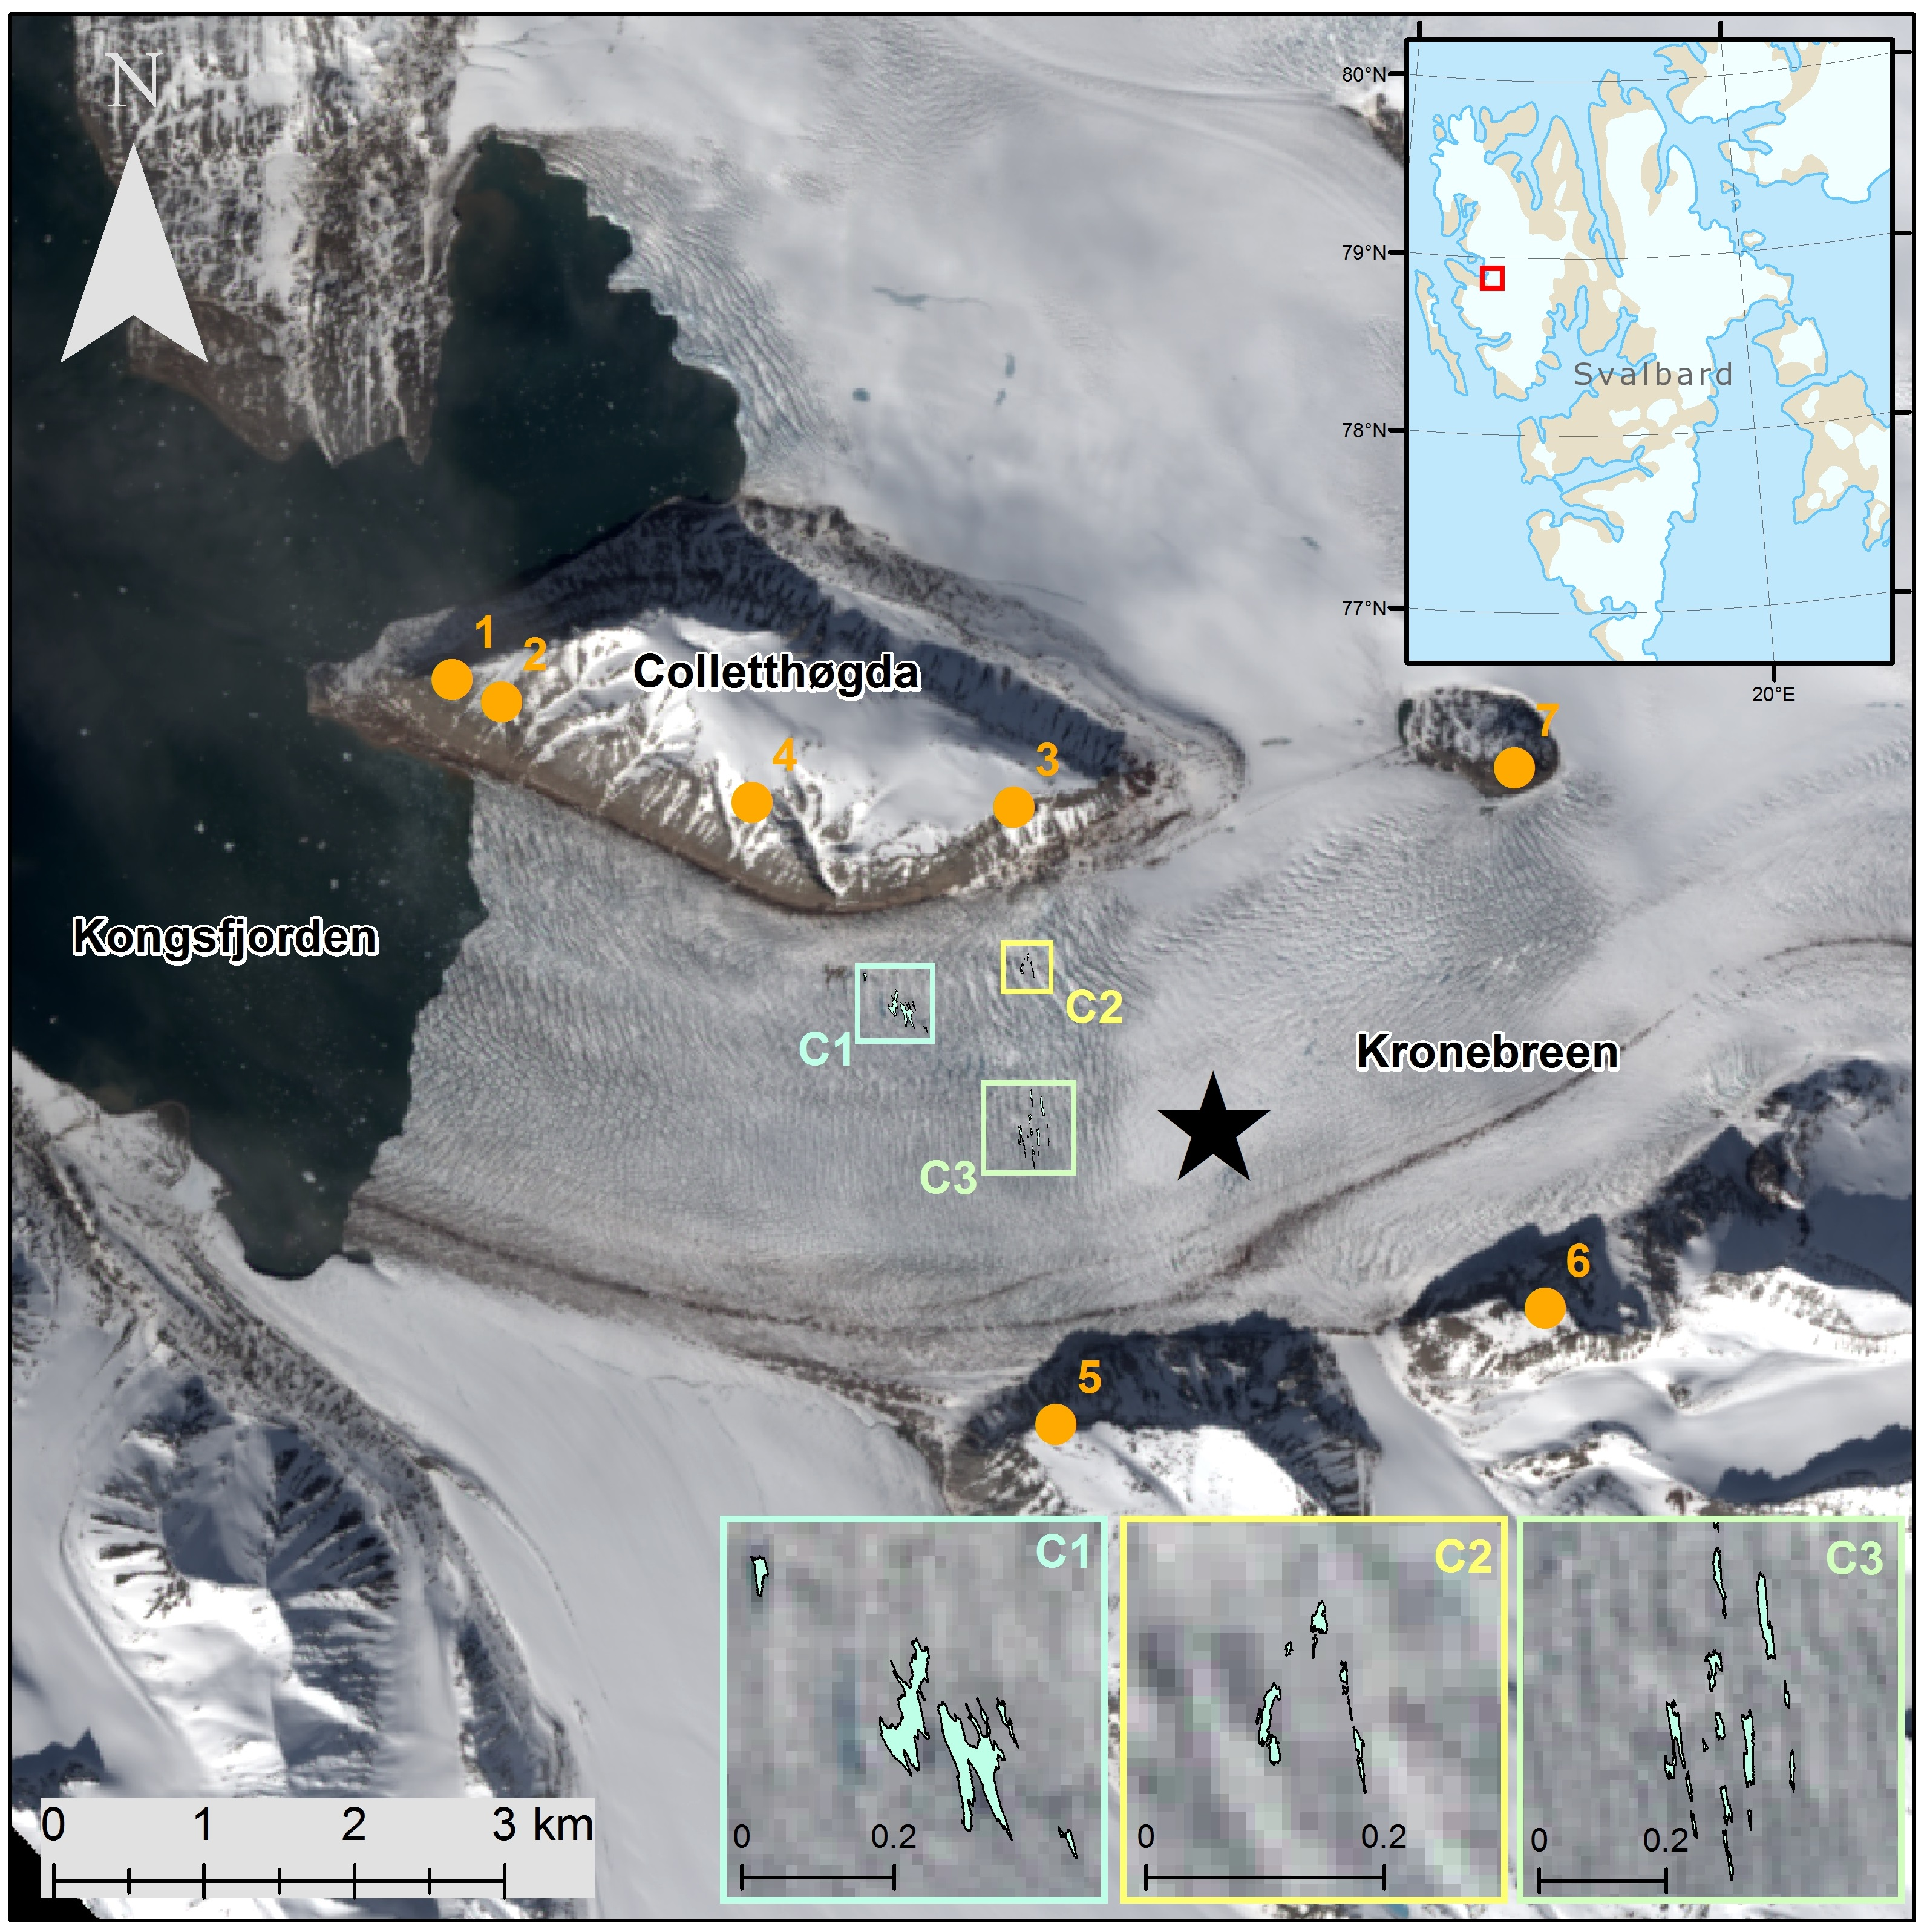
\includegraphics[width=\linewidth]{Chapters/chapter1/figs/examplefigure}
	\caption[Glacier1]{Long description of Glacier by Penny \citep{how_rapidly_2017}}
	\label{fig:examplefigure}
\end{figure}


\chapter{Another chapter}\label{chapter2}
This is an example of another chapter. Much like \ref{chapter1}

% Anything after this line will be an appendix
\appendix
\chapter{TITLE!}
This is an example of an appendix

\begin{table}[h!]
	\centering
	\begin{tabular}{|c|c|}
		\hline 
		\textbf{Pressure (mTorr)} & \textbf{Pressure (Pa)} \\ 
		\hline 
		3.75 & 0.5 \\ 
		7.5 & 1 \\ 
		10 & 1.3 \\ 
		13 & 1.7 \\ 
		20 & 2.7 \\ 
		24 & 3.2 \\ 
		50 & 6.7 \\ 
		60 & 8 \\ 
		64 & 8.5 \\ 
		75 & 10 \\ 
		500 & 66.7 \\ 
		\hline 
	\end{tabular} 
	\caption[Pressures used in this work in mTorr and Pa]{Pressures used in this work in mTorr and Pa.}
\end{table}\label{Appendix1}

% Some people include this, you don't have to but a bit of self promotion never hurt!
%\chapter{List of publications and communications}
%\input{Chapters/Publications/Publications}

% References
\phantomsection
\addcontentsline{toc}{chapter}{List of References}  % Add references to list of contents

% Bibliography style - Harvard is the style requested by Environment
\bibliographystyle{agsm}
\bibliography{references} % .bib file that contains your references (use Jabref, Mendeley, or Endnote etc to manage your references)

\end{document}